\documentclass[12pt]{article}
\usepackage[utf8]{inputenc}
\usepackage{authblk}  % For author affiliations
\usepackage{hyperref} % For hyperlinks
\usepackage{geometry} % For page margins
\usepackage{graphicx} % For including images
\usepackage{amsmath} % For math equation*s
\usepackage{amssymb} % For math symbols
\usepackage{amsthm} % For theorem environments
\usepackage{amsfonts} % For math fonts
\usepackage{mdframed} % For boxes around definitions
\usepackage{mathtools}

% Set definition environment (with box)
\newtheorem{definition}{Definition}[section]
\surroundwithmdframed[
    linewidth=0.5pt,
    innertopmargin=5pt,
    innerbottommargin=5pt,
    skipabove=\baselineskip,
    skipbelow=\baselineskip
]{definition}

\newtheorem{proposition}{Proposition}[section]
\surroundwithmdframed[
    linewidth=0.5pt,
    innertopmargin=5pt,
    innerbottommargin=5pt,
    skipabove=\baselineskip,
    skipbelow=\baselineskip
]{proposition}

\geometry{
    a4paper,
    margin=1in
}

% Set paragraph spacing
\setlength{\parskip}{1.5ex plus 0.5ex minus 0.2ex}

\title{
    An Introduction to Number Theoretic Transform in Post-Quantum Lattice Cryptography \\
    \large EE5163 Advanced Digital Signal Processing: Final Report 
}

\author[1]{
    Lo-Chun, Chou \\
    \small R13922136
}

\affil[1]{Department of Computer Science, National Taiwan University}

\date{\today}

\begin{document}

\maketitle

\begin{abstract}
    In the domain of post-quantum cryptography (PQC), 
    lattice-based cryptography stands out as one of the most promising approaches due to its balanced performance between security and efficiency. 
    A key computational task in these schemes is polynomial multiplication, 
    where Number Theoretic Transform (NTT) is particularly effective for this task. 
    %
    NTT achieves quasilinear time complexity$O(n \log n)$, 
    similar to the Fast Fourier Transform (FFT), 
    but operates entirely over integers, 
    thus avoiding rounding errors from floating-point arithmetic.
    %
    In this report, we explore the foundations of NTT, 
    drawing from some recent research papers, 
    and provide an overview of its principles, implementation strategies, 
    and applications in lattice-based cryptographic systems.
\end{abstract}

\section{Introduction}

\subsection{Motivation}

While both Number Theoretic Transform (NTT) and Fast Fourier Transform (FFT) are used in polynomial multiplication, 
NTT is a relative new approach, which is often not covered in the textbooks. 
This lack of accessible resources is also noted in the reference work 
\emph{A Beginner's Guide to Number Theoretic Transforms (NTTs)}, 
where the authors mentioned that the lack of guidance and tutorial available in one place is the main obstacle for learning NTT\cite{beginner_guide}, 
which is also the reason why they wrote the material.

While the beginner's guide offers a solid introduction to the basic ideas of NTT, 
it occasionally assumes familiarity with advanced mathematical concepts. 
Therefore, we expand upon its foundation by including additional mathematical background, 
clarifying essential concepts such as rings, primitive roots, and modular arithmetic, 
so all mathematical backgrounds that are needed but unfamiliar to a non-math-major would be covered.

Furthermore, 
we conclude with a brief example introducing the applications of NTT in real-world scenarios, 
so that we can move beyond the theoretical part, gaining a full picture of the concept of NTT.

\subsection{Polynomial Multiplication in Cryptographic Systems}

\subsection{Report Structure}

\section{Preliminaries: Mathematical Foundations of the Number Theoretic Transform}

\subsection{Rings and quotient rings}

To properly define primitive roots and illustrate the structure of the Number Theoretic Transform (NTT), 
it is necessary to first introduce the concepts of rings, ideals, and quotient rings. 

These algebraic structures are needed because they provide the foundation for polynomial multiplication in NTT, 
since in order to do polynomial multiplication for polynomials $G(x)$ and $H(x)$, 
both of them must belong to the same quotient ring. 
Due to the fact that quotient rings are constructed on the notions of rings and ideals, 
we begin by briefly reviewing these foundational concepts.

\begin{definition}[Ring, \cite{algebra}, pp.~85--86]
    A set $R$ is called a \textbf{ring} if it has two binary operations, written as addition and multiplication, 
    satisfying the following axioms for all $a, b, c \in R$:
    \begin{enumerate}
        \item $a + b = b + a$.
        \item $a + (b + c) = (a + b) + c$.
        \item An element $0$ in $R$ exists such that $0 + a = a$ for all $a$.
        \item For each $a \in R$ an element $-a \in R$ exists such that $a + (-a) = 0$.
        \item $a(bc) = (ab)c$.
        \item An element $1$ in $R$ exists such that $1 \cdot a = a = a \cdot 1$ for all $a$.
        \item $a (b + c) = ab + ac$ and $(b + c)a = ba + ca$.
    \end{enumerate}
\end{definition}

\begin{definition}[Ideal, \cite{ideal_quotientring}, p.~1]
    A subset $A$ of a ring $R$ (commutative, with $1$) is said to be an \textbf{ideal} if
    \begin{enumerate}
        \item $0 \in A$ and $a, b \in A \Rightarrow a + b, -a \in A$ (so $A$ is an additive subgroup of $R$).
        \item $(a \in A, r \in R)$ $ra \in A$.
    \end{enumerate}
\end{definition}

Intuitively, 
an ideal is a special subset of a ring, 
which includes the zero element and is closed under addition, 
also, it would satisfy that every multiple of an element in $A$ is also in $A$.

\begin{definition}[Quotient Ring, \cite{ideal_quotientring}, p.~3]
    Let $A$ be an ideal in the ring $R$.
    The \textbf{quotient ring} $R/A$ is defined as follows:
    \begin{align*}
        \text{Set} &\coloneq \{r + A \mid r \in R\} \qquad \text{(additive cosets)} \\
        0 &\coloneq A \\
        1 &\coloneq 1 + A \\
        (r + A) + (s + A) &\coloneq (r + s) + A \\
        (r + A)(s + A) &\coloneq (rs) + A \\
    \end{align*}
    where $r, s \in R$.
\end{definition}

To be simple, 
a quotient ring $R/A$ is formed by grouping elements of the ring $R$ into disjoint sets called cosets, 
where each coset has the form $r + A = \{r + a \mid r \in R\}$. 
These cosets partition the ring in a way that reflects the structure of the ideal $A$.

One may wonder why quotient rings are introduced in the literature of NTT.
The idea is that, we treat every element in the same coset as "equivalent", just like in modular arithmetic. 

An important example would be $\mathbb{Z}/n\mathbb{Z}$, which represents the ring of integers modulo $n$, 
where all numbers differed by a multiple of $n$ are considered the same. 
In the same way, a quotient ring allows us to "mod out" an ideal $A$ and treat every element in $A$ as zero, simplifying the structure of the ring and allowing new algebraic manipulations.

To illustrate what this means, 
we can consider the following example:

If given $R = \mathbb{Z}$ and $A = 2\mathbb{Z}$, 
which means that we have the ring of integers and ideal of even numbers, respectively.
Then $R/A = \mathbb{Z}/2\mathbb{Z}$ would be defined as having the set:

\begin{equation*}
    \{r + 2\mathbb{Z} \mid r \in \mathbb{Z}\}
\end{equation*}

Some of its cosets would be:

\begin{align*}
    \{1 + 2\mathbb{Z}\} &= \{1, 3, 5, 7, \ldots\} \\
    \{2 + 2\mathbb{Z}\} &= \{2, 4, 6, 8, \ldots\} \\
    \{3 + 2\mathbb{Z}\} &= \{3, 5, 7, 9, \ldots\} \\
    \vdots
\end{align*}

However, we can see that $\{1 + 2\mathbb{Z}\}$ and $\{3 + 2\mathbb{Z}\}$ are the same, 
thus there would actually be only two cosets:

\begin{align*}
    \{0 + 2\mathbb{Z}\} &= \{0, 2, 4, 6, \ldots\} \\
    \{1 + 2\mathbb{Z}\} &= \{1, 3, 5, 7, \ldots\} 
\end{align*}

Thus, if we have two elements $r_1$ and $r_2$ in the same coset, say $0 + 2\mathbb{Z}$, 
then we can write:

\begin{align*}
    r_1 = 0 + 2 z_1 \quad \text{for some } z_1 \in \mathbb{Z} \\
    r_2 = 0 + 2 z_2 \quad \text{for some } z_2 \in \mathbb{Z}
\end{align*}

and we can see that $r_1 \equiv r_2 \pmod{2\mathbb{Z}}$ since $r_1 - r_2 = 2(z_1 - z_2) \in 2\mathbb{Z}$.
This can also be written as $r_1 - r_2 \equiv 0 \pmod{2\mathbb{Z}}$, and $r_1 - r_2 \in 2\mathbb{Z}$. 
What this means is that, for any element in the ideal $2\mathbb{Z}$, 
it would be treated as equivalent to $0$ in the quotient ring $\mathbb{Z}/2\mathbb{Z}$.

\subsection{Modular Arithmetic and Roots of Unity}

In this subsection, we first introduce the concept of residue class modulo $n$, 
in order to be used in defining $\mathbb{Z}_n$, 
then we further define the order of an integer under modulo $n$, 
so that primitive root can be defined. 
The reason why primitive root is needed is that it is used to construct the NTT matrix, 
which we would talk about the details in the next subsection.

\begin{definition}[Residue Class Modulo $n$, \cite{algebra}, p.~30]
    If $a$ is an integer, its equivalent class $[a]$ with respect to congruence modulo $n$ is called its \textbf{residue class modulo $n$}, 
    and we write $\overline{a} = [a]$ for convenience: 
    \begin{equation*}
    \overline{a} = [a] = \{x \in \mathbb{Z} \mid x \equiv a \pmod{n}\}.
    \end{equation*}
\end{definition}

Intuitively saying, after we selected an integer $n$ to be the modulus, 
we can divide all the integers into $n$ classes, 
each class is a set of integers that having the same remainder when divided by $n$.

Therefore, for any integer $n$, there are $n$ residue classes modulo $n$, 
which are $\overline{0}, \overline{1}, \overline{2}, \ldots, \overline{n - 1}$, 
if we collect all of these residue classes as a set, 
then we get the set of integers modulo $n$, 
which is defined as follows:

\begin{definition}[Integers Modulo $n$, \cite{algebra}, p.~30]
    The set of all residue classes modulo $n$ is denoted 
    \begin{equation*}
    \mathbb{Z}_n = \{\overline{0}, \overline{1}, \overline{2}, \ldots, \overline{n - 1}\}.
    \end{equation*}
    and is called the set of \textbf{integers modulo $n$}.
\end{definition}

Before introducing the definition of primitive root, 
we first define the order of an integer modulo $n$ as follows:

\begin{definition}[Order of an Integer Modulo $n$ , \cite{number_theory}, p.~147]
    Let $n > 1$ and $\gcd(a, n) = 1$. 
    The \textbf{order of $a$ modulo $n$} is the smallest positive integer $k$ such that
    \begin{equation*}
    a^k \equiv 1 \pmod{n}.
    \end{equation*}
\end{definition}

Using the definition of order, we can then define the primitive root as follows:

\begin{definition}[Primitive Root, \cite{number_theory}, p.~150]
    If $\gcd(a, n) = 1$ and $a$ is of order $\varphi(n)$ modulo $n$, 
    then $a$ is called a \textbf{primitive root} of the integer $n$.
    Equivalently, $a$ is a primitive root modulo $n$ if
    \begin{equation*}
    a^{\varphi(n)} \equiv 1 \pmod{n} \quad \text{but} \quad a^k \not\equiv 1 \pmod{n} \quad \forall \ 1 \leq k < \varphi(n).
    \end{equation*}
\end{definition}

Note that the primitive root may not be unique, and since we use the primitive root to construct the NTT matrix, 
the NTT of a polynomial may not be unique and would depend on the choice of the primitive root.
\cite[pp.~5--6]{beginner_guide}
\bigskip

In the context of NTT, we choose the modulus $n$ to be a prime number, let it be denoted as $q$, 
and under the assumption that our polynomials $G(x)$ and $H(x)$ are of degree $n-1$, 
we try to find primitive roots $\omega$ that would satisfy:

\begin{equation*}
    \omega^n \equiv 1 \pmod{q} \quad \text{and} \quad \omega^k \not\equiv 1 \pmod{q} \quad \forall \ 1 \leq k < n.
\end{equation*}

Which means that if we're trying to do convolution of polynomials of degree $3$, 
then we should find a primitive root that would be congruent to $1$ when raised to the power of $4$, 
under some choice of modulus $q$.

And such $\omega$ is called the \textbf{primitive $n$-th root of unity} in the ring $\mathbb{Z}_q$.
\cite[p.~4]{beginner_guide}

\subsection{Cyclotomic Polynomials}

From the previous subsections, we have already defined the quotient ring and the primitive root.
We then introduce the concept of cyclotomic polynomials, 
which is chosen to construct the ideal of the quotient ring.
\cite[p.~3]{survey}

\begin{definition}[Cyclotomic Polynomial, \cite{cyclotomic}, p.~11]
    The $n$-th \textbf{cyclotomic polynomial} $\Phi_n(x)$ is defined by
    \begin{equation*}
        \Phi_n(x) = \prod_{\omega \in P(n)} (x - \omega)
    \end{equation*}
    where $P(n)$ denotes the set of all primitive $n$-th roots of unity.
\end{definition}

But how do we connect the $n$-th cyclotomic polynomial to construct the ideal of the quotient ring?
To answer this question, we first introduce our focus, 
the two widely used rings in lattice-based schemes are:

\begin{equation*}
    \mathbb{Z}_q[x] / (x^n - 1) \quad \text{and} \quad \mathbb{Z}_q[x] / (x^n + 1)
\end{equation*}
\cite[p.~3]{survey}

Here we could see that the ideals of the quotient rings are $(x^n - 1)$ and $(x^n + 1)$, respectively.
To construct these two ideals, we need the following proposition:

\begin{proposition}[Fundamental Relation, \cite{cyclotomic}, p.~12]
    For any positive integer $n$, 
    \begin{equation*}
        x^n - 1 = \prod_{d \mid n} \Phi_d(x)
    \end{equation*}
\end{proposition}

The above proposition shows that, if we are to choose the ideal with the form $(x^n - 1)$, 
then we could construct it by finding all the factors $d$ that could divide $n$, 
then multiply all the $d$-th cyclotomic polynomials together.

To see how this works, we can consider the example of having $n = 4$, 
with the aid of the following table:

\begin{figure}[h]
    \centering
    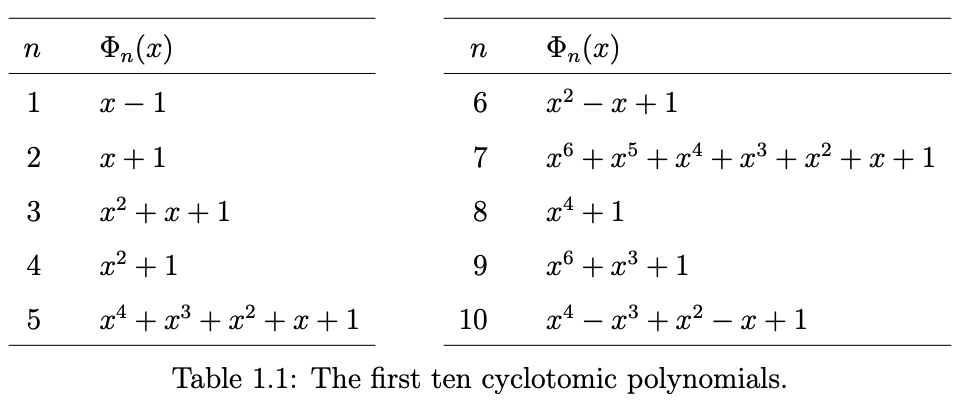
\includegraphics[width=0.8\textwidth]{Final_img/cyclotomic_table.png}
    \caption{Cyclotomic Table. Source: \cite[p.~11]{cyclotomic}}
    \label{fig:cyclotomic_table}
\end{figure}

We can see that, for $n = 4$, 
the factors of $n$ are $1, 2, 4$, 
and the corresponding cyclotomic polynomials are:

\begin{align*}
    \Phi_1(x) &= x - 1 \\
    \Phi_2(x) &= x + 1 \\
    \Phi_4(x) &= x^2 + 1
\end{align*}

According to the fundamental relation, we have:

\begin{align*}
    x^4 - 1 
    &= \prod_{d \mid 4} \Phi_d(x) \\
    &= \Phi_1(x) \Phi_2(x) \Phi_4(x) \\
    &= (x - 1)(x + 1)(x^2 + 1) \\
    &= (x^2 - 1)(x^2 + 1) \\
    &= x^4 - 1
\end{align*}

which matches the result in the table.

This could easily be generalized to the case when we choose the ideal with the form $(x^n + 1)$.
Observe that:

\begin{equation*}
    x^{2n} + 1 = (x^n + 1)(x^n - 1)
\end{equation*}

So we have:

\begin{equation*}
    x^n + 1 = \frac{x^{2n} + 1}{x^n - 1}
\end{equation*}

Using the proposition of the fundamental relation, we have:

\begin{align*}
    x^{2n} - 1 &= \prod_{d \mid 2n} \Phi_d(x) \\
    x^n - 1 &= \prod_{d \mid n} \Phi_d(x) 
\end{align*}

Therefore, we can rewrite the above equation* as:

\begin{equation*}
    x^n + 1 
    = \frac{x^{2n} + 1}{x^n - 1} 
    = \frac{\prod_{d \mid 2n} \Phi_d(x)}{\prod_{d \mid n} \Phi_d(x)}
    = \prod_{d \nmid n, \ d \mid 2n} \Phi_d(x)
\end{equation*}

This means that, if we are to choose the ideal with the form $(x^n + 1)$, 
then we could construct it by finding all the factors $d$ that could divide $2n$ but not $n$, 
then multiply all the $d$-th cyclotomic polynomials together.

In particular, if $n$ is of the special form:

\begin{equation*}
    n = 2^k \qquad \text{for some } k \in \mathbb{N}
\end{equation*}

then we have:

\begin{equation*}
    x^{2^k} + 1 
    = \prod_{d \nmid 2^k, \ d \mid 2^{k+1}} \Phi_d(x)
    = \Phi_{2^{k+1}}(x)
    = \Phi_{2n}(x)
\end{equation*}

Therefore, we arrived at the conclusion that, 
if we are to choose the ideal with the form $(x^n + 1)$ with $n = 2^k, \quad k \in \mathbb{N}$, 
then we could construct it by finding the $2n$-th cyclotomic polynomial $\Phi_{2n}(x)$.

This property is quite useful, so in the context of PQC, 
the chosen ring is mostly $\mathbb{Z}_q[x] / (x^n + 1)$ instead of $\mathbb{Z}_q[x] / (x^n - 1)$.
\cite[p.~8]{beginner_guide} 
And we further denote the $2n$-th root of unity as $\psi$, 
with the detailed definition shown below:

\begin{definition}[$2n$-th Root of Unity, \cite{beginner_guide}, p.~8]
    Let $\mathbb{Z}_q$ be an integer ring modulo $q$, and $n - 1$ is the polynomial degree of $G(x)$ and $H(x)$
    and $\omega$ is the primitive $n$-th root of unity. 
    Define $\psi$ as the \textbf{primitive $2n$-th root of unity} 
    \begin{equation*}
        \iff \psi^2 \equiv \omega \pmod{q} \quad \text{and} \quad \psi^n \equiv -1 \pmod{q}
    \end{equation*}
\end{definition}

With all of these defined, we can then move on to the next section, 
where the definition of the Number Theoretic Transform (NTT) would be introduced based on the above definitions.

\subsection{Notations}

Some of the notations vary across the referenced literature, 
and are modified to maintin the consistency of the notations. 

In this report, we assume that the two given polynomials $G(x)$ and $H(x)$ to be multiplied / convolved, 
are of degree $n-1$ if not specified, which can be written as:

\begin{equation*}
    G(x) = \sum_{i = 0}^{n - 1} G[i] x^i \quad \text{and} \quad H(x) = \sum_{i = 0}^{n - 1} H[i] x^i
\end{equation*}

This can also be represented in the form of a vector:

\begin{equation*}
    G = (G[0], G[1], \ldots, G[n - 1]) \quad \text{and} \quad H = (H[0], H[1], \ldots, H[n - 1])
\end{equation*}

Other notations follow the same convention as in the preliminaries above.

\section{The Number Theoretic Transform (NTT)}

\subsection{Definition of Forward and Inverse NTT}

In the previous subsection, 
we introduced the formulation of the two widely used quotient rings in lattice-based schemes, 
if we focus on the case that the ideal is chosen to be of the form $(x^n + 1)$, 
we then denote them by $R$ and $R_q$, respectively:

\begin{align*}
    R = \mathbb{Z}[x] / (x^n + 1) \quad \text{and} \quad R_q = \mathbb{Z}_q[x] / (x^n + 1)
\end{align*}

Assume the special case where $n = 2^k$, 
and consider $\omega$ to be a primitive $n$-th root of unity in $\mathbb{Z}_q$
which

\begin{equation*}
    \omega^n \equiv 1 \pmod{q} \quad \text{where} \quad q \equiv 1 \pmod{2n}, \ q: \text{prime}, \ n: 2^k 
\end{equation*}

we could define the NTT of a polynomial $G(x) \in R_q$ as:

\begin{equation*}
    \hat{G} = \mathbf{NTT}(G(x)) = \sum_{j = 0}^{n - 1} G[j] \omega^{i j} \pmod{q}
\end{equation*}

Representing in the matrix multiplication form, we have:

\begin{equation*}
    \hat{G} 
    = \mathbf{NTT}(G(x)) 
    = \begin{bmatrix}
        \omega^0 & \omega^0 & \cdots & \omega^0 \\
        \omega^0 & \omega^1 & \cdots & \omega^{n-1} \\
        \omega^0 & \omega^2 & \cdots & \omega^{2(n-1)} \\
        \vdots & \vdots & \ddots & \vdots \\
        \omega^0 & \omega^{n-1} & \cdots & \omega^{(n-1)(n-1)}
    \end{bmatrix}
    \begin{bmatrix}
        G[0] \\
        G[1] \\
        \vdots \\
        G[n-1]
    \end{bmatrix}
\end{equation*}

Note that we previously defined the primitive $2n$-th root of unity $\psi$, 
which satisfies $\psi^2 \equiv \omega \pmod{q}$, hence, 
by plugging $\psi$ into the equation and the matrix above, 
we have:

\begin{equation*}
    \hat{G} = \mathbf{NTT}(G(x)) = \sum_{j = 0}^{n - 1} G[j] \psi^{2 i j} \pmod{q}
\end{equation*}

and the matrix form:

\begin{equation*}
    \hat{G} 
    = \mathbf{NTT}(G(x)) 
    = \begin{bmatrix}
        (\psi^2)^0 & (\psi^2)^0 & \cdots & (\psi^2)^0 \\
        (\psi^2)^0 & (\psi^2)^1 & \cdots & (\psi^2)^{n-1} \\
        (\psi^2)^0 & (\psi^2)^2 & \cdots & (\psi^2)^{2(n-1)} \\
        \vdots & \vdots & \ddots & \vdots \\
        (\psi^2)^0 & (\psi^2)^{n-1} & \cdots & (\psi^2)^{(n-1)(n-1)}
    \end{bmatrix}
    \begin{bmatrix}
        G[0] \\
        G[1] \\
        \vdots \\
        G[n-1]
    \end{bmatrix}
\end{equation*}

And the inverse NTT of $\hat{G}$ is denoted as $\mathbf{NTT^{-1}}(\hat{G})$, 
and defined as:

\begin{equation*}
    G = \mathbf{NTT^{-1}}(\hat{G}) = \sum_{j = 0}^{n - 1} n^{-1} \hat{G}[j] \omega^{-i j} \pmod{q}
\end{equation*}
\cite[p.~4]{fpga}

\subsection{Comparison with Fast Fourier Transform (FFT)}

% Consider a periodic sequence $x[n]$ with period $N$ and with the Fourier series representation:

% \begin{equation*}
%     x[n] = \sum_{k = \langle N \rangle} a_k e^{j \frac{2 \pi}{N} k n}
% \end{equation*}

% Suppose we choose the interval of summation above to be $k = 0, 1, \ldots, N - 1$, 
% then we have:

% \begin{equation*}
%     x[n] = a_0 + a_1 e^{j \frac{2 \pi}{N} n} + a_2 e^{j \frac{2 \pi}{N} 2 n} + \cdots + a_{N-1} e^{j \frac{2 \pi}{N} (N-1) n}
% \end{equation*}

From the Cooley-Tukey algorithm \cite[p.~370]{ADSP5}, 
we recall that the DFT of a sequence $x[n]$ of length $N = 2^k$ is given by:

\begin{align*}
    X[m] 
    &= \sum_{n = 0}^{N - 1} x[n] e^{-j \frac{2 \pi m n}{N}} \\
    &= \sum_{n = 0}^{N/2 - 1} x[2n] e^{-j \frac{2 \pi m (2n)}{N}} + \sum_{n = 0}^{N/2 - 1} x[2n + 1] e^{-j \frac{2 \pi m (2n + 1)}{N}} \\
    &= \sum_{n = 0}^{N/2 - 1} x[2n] e^{-j \frac{2 \pi m n}{N/2}} + \underbrace{e^{-j \frac{2 \pi m}{N}}}_{\text{twiddle factors}} \sum_{n = 0}^{N/2 - 1} x[2n + 1] e^{-j \frac{2 \pi m n}{N/2}} 
\end{align*}

where the second equality is by splitting the summation into two parts, 
one for the even-indexed terms and the other for the odd-indexed terms, 
then they could further be derived into two $\frac{N}{2}$-point DFTs, with twiddle factor $e^{-j \frac{2 \pi m}{N}}$.

Since NTT is DFT in another ring, we could also apply similar techniques as in the Cooley-Tukey algorithm to optimize NTT, 
making the original complexity of NTT from $O(n^2)$ to $O(n \log n)$. 
This is achieved by utilizing the two properties of the primitive $2n$-th root of unity $\psi$ \cite[p.~11]{beginner_guide}:

\begin{align*}
    \text{periodicity:}& \quad \psi^{k + 2n} = \psi^k \\
    \text{symmetry:}& \quad \psi^{k + n} = -\psi^k \qquad \text{where } k \in \mathbb{Z}^+
\end{align*}

By these properties, 
we could divide the calculation of $n$-point NTT and INTT into two $\frac{n}{2}$-point NTT and INTT, 
similar to what we have done in the DFT case as below:

\begin{align*}
    \hat{G} 
    &= \mathbf{NTT}(G(x)) \\
    &= \sum_{j = 0}^{n - 1} G[j] \psi^{2 i j} \pmod{q} \\
\end{align*}

Split the summation into even and odd indices:

\begin{align*}
    \hat{G} 
    &= \sum_{j = 0}^{n - 1} G[j] \psi^{2 i j} \pmod{q} \\
    &= \sum_{i = 0}^{n/2 - 1} \psi^{2j(2i) + 2i} G[2i] + \sum_{i = 0}^{n/2 - 1} \psi^{2j(2i+1) + 2i+1} G[2i+1] \pmod{q} \\
    &= \sum_{i = 0}^{n/2 - 1} \psi^{4ij + 2i} G[2i] + \psi^{2j + 1} \sum_{i = 0}^{n/2 - 1} \psi^{4ij + 2i} G[2i+1] \pmod{q}
\end{align*}

Define:

\begin{equation*}
    A_j = \sum_{i = 0}^{n/2 - 1} \psi^{4ij + 2i} G[2i], \quad B_j = \sum_{i = 0}^{n/2 - 1} \psi^{4ij + 2i} G[2i+1]
\end{equation*}

We then express the result as:

\begin{equation*}
    \hat{G}_j = A_j + \psi^{2j + 1} B_j \pmod{q}
\end{equation*}

Next, using the symmetry property $\psi^{k + n} \equiv -\psi^k \pmod{q}$, we can derive:

\begin{equation*}
    \hat{G}_{j + n/2} = A_j - \psi^{2j + 1} B_j \pmod{q}
\end{equation*}

Thus, we obtain the fast-NTT update rules:

\begin{align*}
    \hat{G}_j &= A_j + \psi^{2j+1} B_j \pmod{q} \\
    \hat{G}_{j + n/2} &= A_j - \psi^{2j+1} B_j \pmod{q}
\end{align*}

This is structurally identical to the radix-2 butterfly unit in FFT, 
replacing the complex twiddle factor $e^{-j\frac{2\pi}{N}m}$ with integer twiddle factors $\psi^{2j+1}$ in $\mathbb{Z}_q$.

\subsection{Types of Convolutions and Equivalent NTTs}


\section{Limitations of NTT}

\subsection{Parameter Restrictions and Ring Compatibility}

\subsection{Negative Wrapped Convolution and Modulus Conditions}

\subsection{Hardware Bottlenecks and Communication Overheads}

In hardware implementations of the Number Theoretic Transform (NTT), 
one major source of inefficiency arises from the intricate data communication between adjacent computation stages. 

\begin{figure}[h]
    \centering
    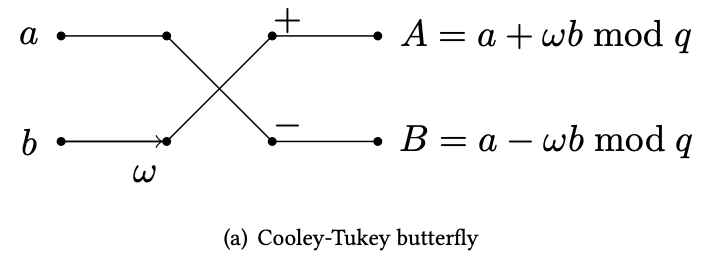
\includegraphics[width=0.8\textwidth]{Final_img/CT_butterfly.png}
    \caption{Butterfly Diagram of the Cooley–Tukey NTT Algorithm. Source: \url{https://k.rypto.cafe/assets/images/misc/ct_butterfly.png}}
    \label{fig:butterfly}
\end{figure}

As visualized in the butterfly diagram of the Cooley–Tukey NTT algorithm, 
multiple stages are required to process even small-length inputs, 
and each stage introduces data dependencies that result in extensive data movement. 
This leads to increased wiring complexity and higher area and energy overhead when deploying NTT on ASIC or FPGA-based accelerators. 
For in-memory computing architectures, 
these inefficiencies translate into additional shift operations to align data with memory bitlines, 
further increasing latency and hardware cost.


\subsection{Handling NTT-Unfriendly Rings and Algorithmic Alternatives}

\section{Applications of NTT in Lattice-Based Cryptography}

\subsection{NTT in Post-Quantum Cryptographic Schemes}

\subsection{Error-Resilient and Hardware-Efficient Implementations}

\subsection{Optimized NTT Variants for Real-World Schemes}

\section{Conclusion and Future Directions}

\subsection{Summary of Key Concepts}

\subsection{Challenges and Open Research Problems}






\bibliographystyle{plain}
\bibliography{ADSP_final_ref} 

\end{document} 